\section{Inserción}
Para insertar un nodo en el Octree llamamos la función recursiva \verb!insert! para almacenar un punto (esfera) en el octree.

Si no está contenido buscamos otro octante. Si nos encontramos en el octante, verificamos que la capacidad no se halla rebasado, sí este fuera el caso dividimos en ocho octantes.\cite{samet}.
\begin{lstlisting}[caption=El método Insert(point)]
  insert(point) {
    //Si el punto no esta en los limites (cubo)del octree Return
    if (!this.cubo.contains(point)) {
      return false;
    }
    //Si ( this . points . length ) < ( this . capacity )
    if (this.points.length < this.capacity) {
      //Insertamos en el vector this . points
      this.points.push(point);
      //Color a la esfera
      point.material.color.set(this.color);
      return true;

    }
    else {
      //Dividimos si aun no ha sido dividido
      if (!this.divided) {
        this.subdivide();
      }
      //Insertamos recursivamente en los 8 hijos
      this.northeastf.insert(point);
      this.northwestf.insert(point);
      this.southeastf.insert(point);
      this.southwestf.insert(point);
      this.northeastb.insert(point);
      this.northwestb.insert(point);
      this.southeastb.insert(point);
      this.southwestb.insert(point);
    }
  }
\end{lstlisting}

A continuación se muestran algunos ejemplos:
\begin{itemize}
    \item Inserción de un punto (esfera)
    \begin{figure}[H]
      \centering
      \fbox{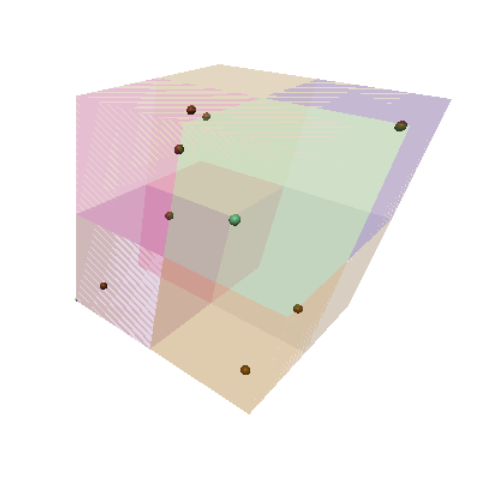
\includegraphics[width=0.55\textwidth]{insert01}}
      \caption{Relación en color del dato (punto) con el nodo (octante) al que pertenece.}
      \label{fig:insert01}
    \end{figure}
    \item Inserción de una cantidad determinada en coordenadas aleatorias
    \begin{figure}[H]
      \centering
      \fbox{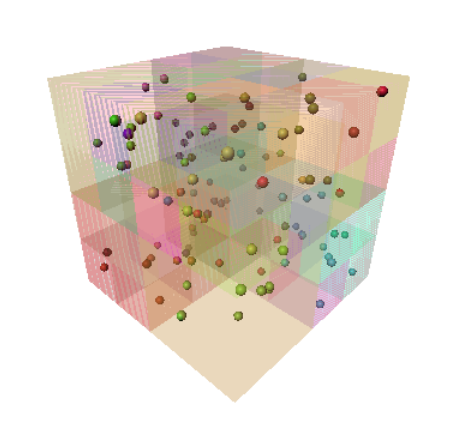
\includegraphics[width=0.55\textwidth]{insert02}}
      \caption{Inserción de puntos en coordenadas aleatorias}
      \label{fig:insert02}
    \end{figure}
\end{itemize}

\subsection{El método subdivide}
Divide el octree:
\begin{lstlisting}
  //divide el octree en 8 octrees
  subdivide() {
    let x = this.cubo.x;
    let y = this.cubo.y;
    let z = this.cubo.z;
    let w = this.cubo.w / 2;
    let h = this.cubo.h / 2;
    let d = this.cubo.d / 2;

    // Crear 8 hijos
    let nef = new Cubo(x + w, y - h, z - d, w, h, d);
    let nwf = new Cubo(x - w, y - h, z - d, w, h, d);
    let sef = new Cubo(x + w, y + h, z - d, w, h, d);
    let swf = new Cubo(x - w, y + h, z - d, w, h, d);

    let neb = new Cubo(x + w, y - h, z + d, w, h, d);
    let nwb = new Cubo(x - w, y - h, z + d, w, h, d);
    let seb = new Cubo(x + w, y + h, z + d, w, h, d);
    let swb = new Cubo(x - w, y + h, z + d, w, h, d);

    //Asignar los OcTree creados a cada hijo
    this.northeastf = new OcTree(nef, this.capacity);
    this.northwestf = new OcTree(nwf, this.capacity);
    this.southeastf = new OcTree(sef, this.capacity);
    this.southwestf = new OcTree(swf, this.capacity);

    this.northeastb = new OcTree(neb, this.capacity);
    this.northwestb = new OcTree(nwb, this.capacity);
    this.southeastb = new OcTree(seb, this.capacity);
    this.southwestb = new OcTree(swb, this.capacity);


    //Hacer : this . divided <- true
    this.divided = true;

  }  
\end{lstlisting}





\iffalse
% ---- Para poner dos imágenes (una a lado de otra) ----
Como se muestra en la figuras \ref{fig:act-1_a} y \ref{fig:act-1_b}.
\begin{figure}[H]
\centering
\begin{minipage}{0.45\textwidth}
  \centering
  \includegraphics[width=0.9\textwidth]{act-1_a}
  \caption{Envío de \textit{ICMP ECHO REQUEST} de PC0 a PC1, PC2 y PC3.}
  \label{fig:act-1_a}
\end{minipage}\hfill
\begin{minipage}{0.45\textwidth}
  \centering
  \includegraphics[width=0.9\textwidth]{act-1_b}
  \caption{Respuesta de PC1, PC2 y PC3. Tabla ARP de PC0.}
  \label{fig:act-1_b}
\end{minipage}
\end{figure}
% ---- Para colocar una imagen ----
Como se muestra en la figura \ref{fig:act-3}
\begin{figure}[H]
  \centering
  \includegraphics[width=0.8\textwidth]{act-3}
  \caption{Tabla de subneteo para la red 192.168.100.0.}
  \label{fig:act-3}
\end{figure}
\fi